\chapter{Final Prototype}

The current DORI prototype is shown in Fig.~\ref{fig:prototype}.
A new PCB was designed with emphasis on a more compact footprint, correcting the layout errors identified in the DORI-test board and optimised for wireless operation. In comparison with the previous PCB, the colour-coded LED was integrated, and a power switch was added to disconnect the LiPo battery from the circuit. Additionally, all oscilloscope test points were removed and the SiPM is now soldered directly onto the board.

To obtain a portable version of the system, and to ensure that no ambient light reaches the photosensitive elements, a two-part 3D printed case was designed. The lower layer contains a dedicated compartment for the LiPo battery (Fig.~\ref{fig:prototype}~(a)) and is enclosed by the PCB. As shown in Fig.~\ref{fig:prototype}~(b), the PS was wrapped in several layers of Teflon tape, covering all non-exiting surfaces of the cube. Optical silicone grease(!!!!!!!) was applied as coupling between the SiPM and the PS. The friction it creates, together with dedicated holes in the top layer of the case, keep the PS in place and aligned with the SiPM. Apertures are provided for the LED, the power switch (Fig.~\ref{fig:prototype}~(c)) and the USB-C port for charging and firmware uploading. The top layer is closed tightly against the bottom one with four screws. A loop was modelled on the top to hold a standard badge clip, allowing the unit to be worn over clothing. As represented, the current DORI unit measures 6.3~cm in width, 7.2~cm in height and 2.5~cm in thickness, with a total mass of 141~g. For comparison, the RaySafe i3 device measures 4.0 $\times$ 5.8 $\times$ 1.7~cm and has a mass of only 34~g. Although the dimensions are comparable, the DORI PCB still leaves room for improvement in size, through a better use of the PCB's top and bottom layers for component placement. Additionally, the integration of the ESP32-C3 as a bare chip, rather than the prototyping module, would contribute further to the reduction of the footprint. From a wearable point of view, the mass is currently the most likely cause of discomfort. The enclosure was printed at 100\% infill to guarantee that no ambient light reaches the photosensitive elements. This choice increases the mass of the unit, which is higher than desirable for a badge worn over clothing. If light-tightness can be preserved, a reduction can be achieved with a lower infill density, or with different printing methods and materials.

All design files of the final prototype are made available in a public repository [repository link], so that the system can be reproduced and further developed. These include the CAD models of the enclosure, the PCB layout and schematic, the firmware, the acquisition software and the energy and dose calibration parameters derived in this work. Future work should also include the implementation of the graphical user interface projected in Chapter~\ref{chapter:hardware_development}, for real time visualisation of the dose rate and storage of the acquired data.

\begin{figure}[H]
  \centering
  \resizebox{1\linewidth}{!}{\begin{tikzpicture}[x=1pt,y=1pt,
    every node/.style={font=\footnotesize},
    ah/.style={draw opacity=0,line width=0.08,fill opacity=1},
    ahs/.style={ah,scale=0.55},
    lbl/.style={fill=white,align=center,inner sep=2.5pt,line width=0.6pt},
    dim/.style={fill=white,align=center,inner sep=2pt,draw=none,font=\scriptsize},
    pan/.style={font=\footnotesize\bfseries,inner sep=0pt,anchor=north}]

% =========================================================================
% (a)  bottom shell  --  image x: 59.5 -> 237.25 , y: 172 -> 308.9
% =========================================================================
\node [anchor=south west,inner sep=0] at (59.5,172)
  {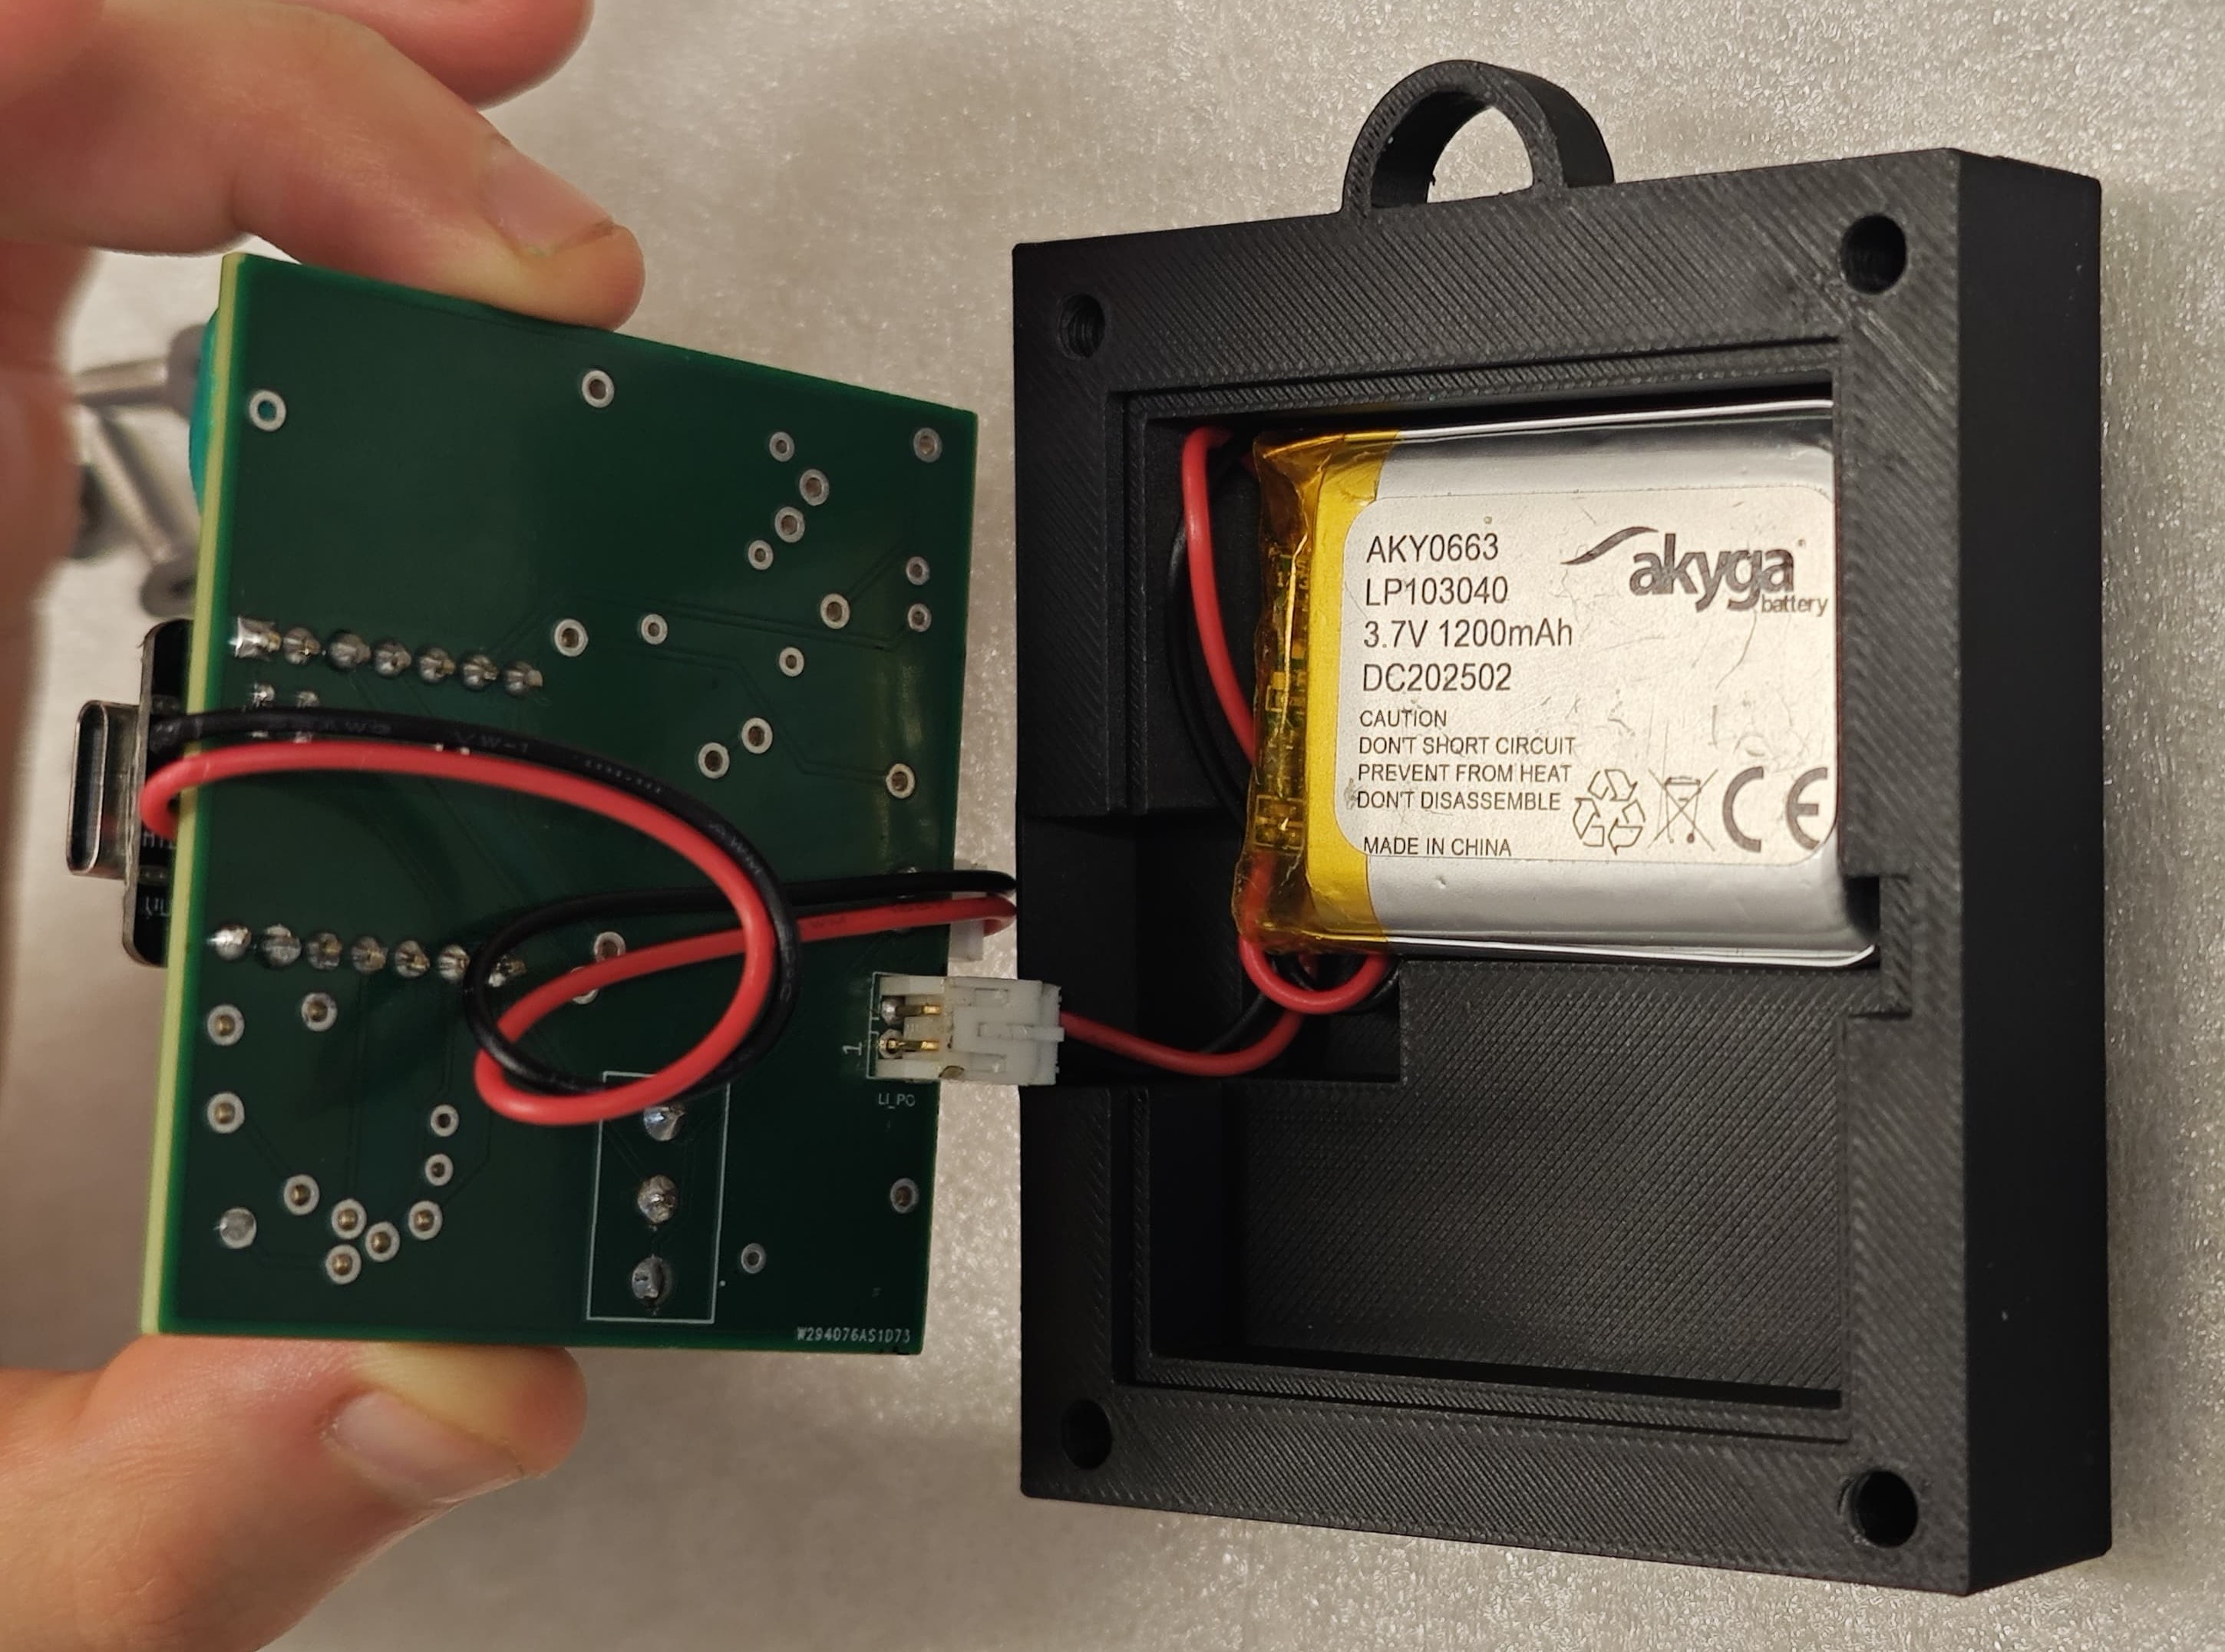
\includegraphics[width=177.75pt,height=136.9pt]{images/baixo.jpg}};

% ---- Battery + cables compartment ---------------------------------------
\node [lbl,draw={rgb, 255:red, 81; green, 81; blue, 81 },anchor=center]
      (batt) at (106.1,280.6) {Battery + Cables\\Compartment};
\draw [color={rgb, 255:red, 81; green, 81; blue, 81 },line width=1.1pt]
      ([xshift=12.5pt]batt.south) -- (147.0,240.4);
\draw [shift={(152.6,234.7)},rotate=134.3,ah,
       fill={rgb, 255:red, 81; green, 81; blue, 81 }]
      (7.85,-3.78) -- (0,0) -- (7.85,3.78) -- cycle ;

% ---- Power cables -------------------------------------------------------
\node [lbl,draw={rgb, 255:red, 241; green, 74; blue, 64 },anchor=center]
      (pcab) at (163.25,189.1) {Power\\Cables};
\draw [color={rgb, 255:red, 241; green, 74; blue, 64 },line width=1.1pt]
      ([xshift=-8pt]pcab.north) -- (151.0,213.7);
\draw [shift={(148.6,221.35)},rotate=287.4,ah,
       fill={rgb, 255:red, 241; green, 74; blue, 64 }]
      (7.85,-3.78) -- (0,0) -- (7.85,3.78) -- cycle ;
\draw [color={rgb, 255:red, 241; green, 74; blue, 64 },line width=1.1pt]
      ([xshift=-8pt]pcab.north) -- (126.4,217.7);
\draw [shift={(119.6,221.85)},rotate=328.6,ah,
       fill={rgb, 255:red, 241; green, 74; blue, 64 }]
      (7.85,-3.78) -- (0,0) -- (7.85,3.78) -- cycle ;

% ---- Panel letter (centred on the image) --------------------------------
\node [pan] at (148.375,164) {(a)};
\begin{scope}[yshift=8pt]
% =========================================================================
% (b)  middle shell  --  image x: 0 -> 135.7 , y: 0 -> 146
% =========================================================================
\node [anchor=south west,inner sep=0] at (0,0)
  {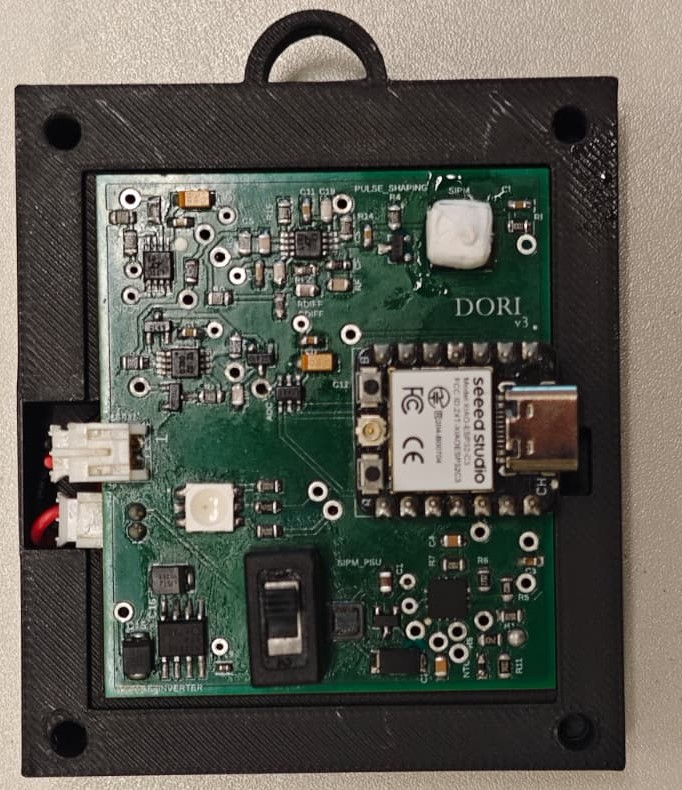
\includegraphics[width=135.7pt,height=146pt]{images/meio.jpg}};

% ---- Teflon-wrapped scintillator ---------------------------------------
\node [lbl,draw={rgb, 255:red, 26; green, 111; blue, 223 },anchor=center]
      (tefl) at (56.65,126.2) {Teflon-wrapped\\Scintillator};
\draw [color={rgb, 255:red, 26; green, 111; blue, 223 },line width=1.1pt]
      ([xshift=9.35pt]tefl.south) -- (79.2,107.0);
\draw [shift={(86.0,102.8)},rotate=148.2,ah,
       fill={rgb, 255:red, 26; green, 111; blue, 223 }]
      (7.85,-3.78) -- (0,0) -- (7.85,3.78) -- cycle ;

% ---- Width dimension (6.3 cm) ------------------------------------------
\draw [line width=1.1pt,black] (2,-4) -- (123.5,-4);
\draw [shift={(2,-4)},rotate=0,ah,fill=black]
      (7.85,-3.78) -- (0,0) -- (7.85,3.78) -- cycle ;
\draw [shift={(123.5,-4)},rotate=180,ah,fill=black]
      (7.85,-3.78) -- (0,0) -- (7.85,3.78) -- cycle ;
\node [dim,anchor=center] at (62.8,-4) {6.3~cm};
% ---- Height dimension (7.2 cm) -----------------------------------------
\draw [line width=1.1pt,black] (-4,3.5) -- (-4,132.5);
\draw [shift={(-4,3.5)},rotate=90,ah,fill=black]
      (7.85,-3.78) -- (0,0) -- (7.85,3.78) -- cycle ;
\draw [shift={(-4,132.5)},rotate=270,ah,fill=black]
      (7.85,-3.78) -- (0,0) -- (7.85,3.78) -- cycle ;
\node [dim,anchor=center,rotate=90] at (-4,68) {7.2~cm};

% ---- Panel letter -------------------------------------------------------
\node [pan] at (67.85,-10) {(b)};

% =========================================================================
% (c)  top shell  --  image x: 159.7 -> 296.8 , y: 0 -> 146
% =========================================================================
\node [anchor=south west,inner sep=0] at (159.7,0)
  {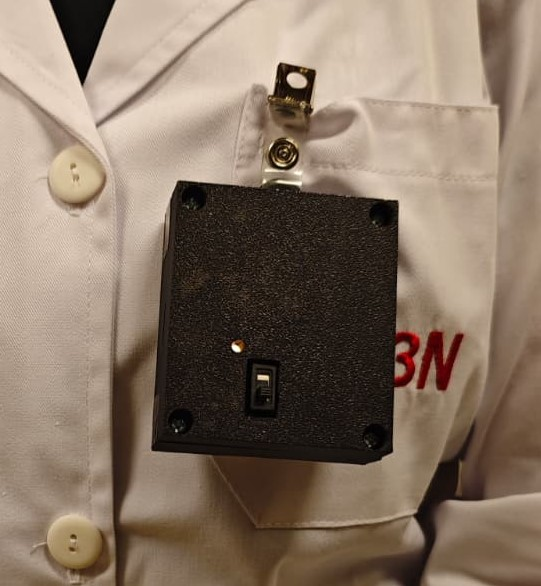
\includegraphics[width=137.1pt,height=146pt]{images/cima.jpg}};
% ---- LED --------------------------------------------------------------
\node [lbl,draw={rgb, 255:red, 204; green, 153; blue, 0 },anchor=center]
      (led) at (181.75,71.45) {LED On};
\draw [color={rgb, 255:red, 204; green, 153; blue, 0 },line width=1.1pt]
      (led.east) -- (217.6,61.6);
\draw [shift={(219.5,60.4)},rotate=151.2,ah,
       fill={rgb, 255:red, 204; green, 153; blue, 0 }]
      (7.85,-3.78) -- (0,0) -- (7.85,3.78) -- cycle ;
% ---- Badge clip ---------------------------------------------------------
\node [lbl,draw={rgb, 255:red, 55; green, 173; blue, 107 },anchor=center]
      (badge) at (269.4,107.7) {Badge Clip};
\draw [color={rgb, 255:red, 55; green, 173; blue, 107 },line width=1.1pt]
      (badge.north) -- (245.3,120.7);
\draw [shift={(237.5,122.6)},rotate=346.6,ah,
       fill={rgb, 255:red, 55; green, 173; blue, 107 }]
      (7.85,-3.78) -- (0,0) -- (7.85,3.78) -- cycle ;


% ---- Power switch -------------------------------------------------------
\node [lbl,draw={rgb, 255:red, 241; green, 74; blue, 64 },anchor=center]
      (psw) at (265.15,47) {Power\\Switch};
\draw [color={rgb, 255:red, 241; green, 74; blue, 64 },line width=1.1pt]
      (psw.west) -- (240,47);
\draw [shift={(232,47)},rotate=0,ah,
       fill={rgb, 255:red, 241; green, 74; blue, 64 }]
      (7.85,-3.78) -- (0,0) -- (7.85,3.78) -- cycle ;

% ---- Thickness dimension (2.5 cm, short arrow -> scaled heads) ----------
\draw [line width=1.1pt,black] (201.0,92.9) -- (205.8,101.6);
\draw [shift={(201.0,92.9)},rotate=61.1,ahs,fill=black]
      (7.85,-3.78) -- (0,0) -- (7.85,3.78) -- cycle ;
\draw [shift={(205.8,101.6)},rotate=241.1,ahs,fill=black]
      (7.85,-3.78) -- (0,0) -- (7.85,3.78) -- cycle ;
\node [dim,anchor=center,rotate=61] at (194.7,102.2) {2.5~cm};
% ---- Panel letter -------------------------------------------------------
\node [pan] at (228.25,-10) {(c)};
\end{scope}
\end{tikzpicture}}
  \caption[Final DORI prototype.]{Final DORI prototype. \textbf{(a)} Bottom layer of
the enclosure, with the compartment holding the LiPo battery and the cables that
connect it to the board. \textbf{(b)} Assembled PCB, with
the Teflon-wrapped scintillator coupled to the SiPM. \textbf{(c)} Closed prototype
worn over a lab coat, with the badge clip, the power switch and the LED on.}
  \label{fig:prototype}
\end{figure}

\section{Channel Response}
\label{sec:channel_response}

Although the readout circuit is the one described in Section~\ref{sec:front_end}, the response of the new prototype cannot be assumed to be that of the DORI-test board. Component values are specified within tolerance bands, and the parasitic contributions and noise coupling introduced by a board are a property of its layout. Both act on the final amplitude at the sampling stage, and consequently on the channel at which a given deposited energy is recorded. Characterising this response allows the front-end design to be treated as transferable and scalable to different board dimensions and formats. If the response of a new board can be related to that of the fully characterised DORI-test board, then the same readout can be used in whatever format each proposed monitoring position demands. 

To verify this, the \emph{Bremsstrahlung} endpoint procedure of Section~\ref{sec:energy_calibration} was repeated. Spectra were acquired over 5-minute intervals for tube voltages of 20 to 50~kVp, at tube currents of 0.100, 0.150 and 0.200~mA. The endpoint channel was extracted from each acquisition as before. The detector was again positioned within the beam line, although at a distance different from the one used previously. The change was required to prevent saturation of the front-end electronics across the full range of tube voltages, and it is the reason why no spectrum was obtained at 20~kVp. At this distance and fluence the counts registered at that voltage remain within the excluded background. A shorter distance or a higher tube current would recover the point at the cost of saturating the front end at the upper voltages. Additionally, the 3D printed case adds absorption, most significantly at the lower energies. The resulting endpoint channels are summarised in Table~\ref{tab:endpoints_prototype}. The uncertainty on the individual endpoints follows the pattern already described for the energy calibration. At 25~keV it is dominated by counting statistics, it decreases towards the middle of the interval. It increases again towards 50~keV, where photoelectric absorption in the scintillator drops and pile-up distorts the spectral shape near the abscissa.
% Requires \usepackage{tabularx} in the preamble

% Small vertical space after surrounding text
\vspace{1em}

% Manual table title, numbered and added to LoT
\refstepcounter{table}
\label{tab:endpoints_prototype}
\noindent\textbf{Table~\thetable.} \emph{Bremsstrahlung} endpoint channel for each tube voltage, obtained with the final prototype. Values are the mean of three acquisitions with the maximum deviation from the mean.
\addcontentsline{lot}{table}{\protect\numberline{\thetable}\emph{Bremsstrahlung} endpoint channel for each tube voltage, obtained with the final prototype.}

% Small space between title and table
\vspace{0.1em}

\begin{table}[H]
  \centering
  \begin{tabularx}{\textwidth}{>{\centering\arraybackslash}m{0.18\textwidth}
                               *{6}{>{\centering\arraybackslash}X}}
    \toprule
    \scriptsize \textbf{Tube Voltage (kVp)} & \scriptsize \textbf{25} & \scriptsize \textbf{30} & \scriptsize \textbf{35} & \scriptsize \textbf{40} & \scriptsize \textbf{45} & \scriptsize \textbf{50} \\
    \midrule
    \scriptsize \textbf{Endpoint Channel (a.u.)}
    & \scriptsize $30 \pm 4\%$
    & \scriptsize $34 \pm 1\%$
    & \scriptsize $36 \pm 1\%$
    & \scriptsize $39 \pm 1\%$
    & \scriptsize $41 \pm 1\%$
    & \scriptsize $42 \pm 2\%$ \\
    \bottomrule
  \end{tabularx}
\end{table}

 The endpoints obtained with the final prototype are presented against those of the test board at the same tube voltages in Fig.~\ref{fig:channel_response}. A linear fit was applied, and with $R^2 = 0.998$ a correspondence between the two boards can be expressed. The slope of the fit is $1.01 \pm 0.02$. This parameter translates the gain of the readout chain. If the two boards differed in gain, every channel would be scaled by a common factor, different from one, as the energy increased. The slope obtained is one within its uncertainty, so the gain is preserved on the new board, within the tolerance of the components that set it. The fit does not, however, pass through the origin. Comparing the endpoints of Tables~\ref{tab:endpoints_prototype} and~\ref{tab:endpoints} directly, the final prototype records every event $3.0 \pm 0.2$ channels below the test board, consistent with the intercept of the fit. With a unit slope, this displacement is the same at every energy of the interval. A difference that does not grow with the signal is additive, and corresponds to a baseline shift, in which all pulses are sampled from a level slightly lower than on the test board. With a channel width of 3.2~mV, three channels correspond to approximately 9.6~mV of shift, introduced at some point at the output of the shaper. The consequence for the calibration is direct as only the intercept changes. The slope of Eq.~\ref{eq:energy_conversion} is retained, since the gain is preserved, and $b$ is displaced by the constant offset. The calibration established for the DORI-test board therefore applies to the final prototype, and the energy of an event can be obtained from its channel simply through a conversion factor. Although the 20~kVp point could not be measured and the $^{241}$Am measurements were not repeated, the 20 to 60~keV range is still preserved, as long as the channels are corrected by the offset, as the response was shown to be linear in Section~\ref{sec:energy_calibration}.

 \begin{figure}[H]
  \centering
  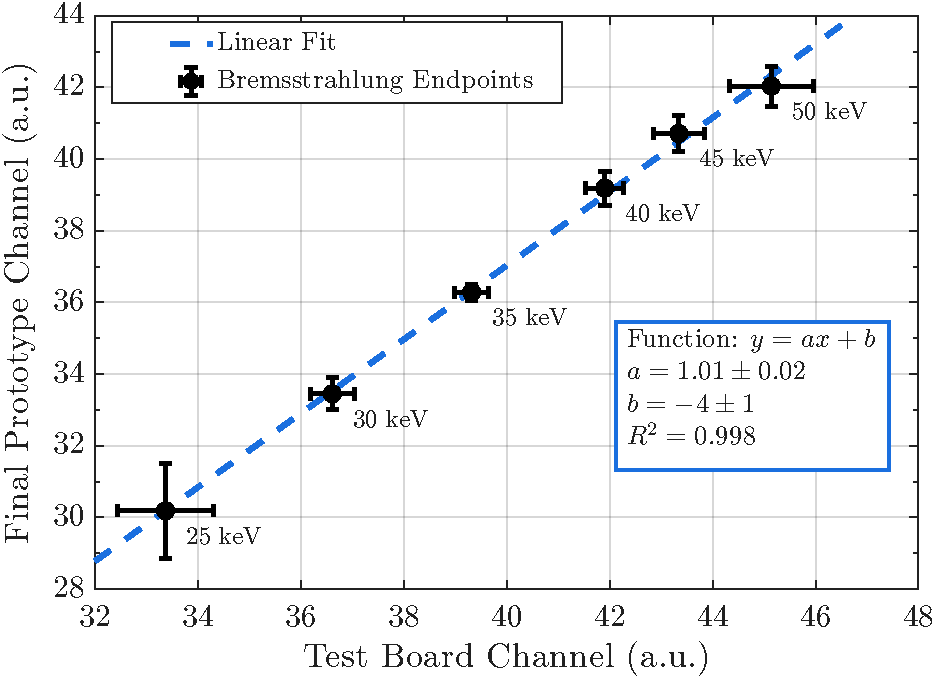
\includegraphics[width=0.85\linewidth]{images/channel_transfer.pdf}
  \caption[Endpoint channel correspondence between the DORI-test board and the final prototype.]{%
Linear fit of the \emph{Bremsstrahlung} endpoint channels recorded by the final
 prototype against those recorded by the DORI-test board, for the tube voltages common to both acquisitions.
  }
  \label{fig:channel_response}
\end{figure}


\section{Power Consumption}
\label{sec:power_consumption}
As a final test, and with a PCB optimised for wireless communication, the power consumption of the current DORI electronics and firmware was analysed. The battery was fully charged through the USB-C connector of the ESP32-C3, the end of the charge being indicated by the red LED of the MCU turning off, and a simulation firmware was
uploaded. One hundred interrupts (events) per second were simulated, and the battery voltage was read with \texttt{analogRead} through a voltage divider connected to the battery terminals. The event data were transmitted over BLE at a one second rate, and the battery voltage was recorded every 15 minutes. A cutoff was added at 3.3 V, at which the MCU is sent into deep sleep in order to preserve the LiPo cell from a full discharge. 

DORI operated for approximately 8.6 hours before the cutoff was reached, at a mean discharge rate of 80 mV/h. For the 1200 mAh cell used, this corresponds to a mean current of approximately 140 mA at 3.7 V. While this is sufficient for uninterrupted operation over an eight hour working day, it would require frequent charging cycles. Thefore, there is still room for improvement in the component selection of the DORI board with respect to consumption. Nevertheless, the battery voltage is a poor indicator of the charge remaining, and a proper characterisation of the cell would be required before it could be used to estimate the current state of charge.
Additionally, the integrity of the wireless link was kept intact throughout the run, with no disconnections and no lost notifications. No rise was registered in the temperature of the MCU, indicating that no thermal load builds up even after continuous hours of operation.

\section{Cost and Specifications}
\label{sec:cost_specifications}

DORI is also intended to represent a more cost effective solution against the prices currently charged for the active devices mentioned in the introduction. An estimated cost of the current prototype is listed in Table~\ref{tab:cost}, excluding assembly and the marginal cost of consumables. The detection chain accounts for most of the total, with the scintillator and the SiPM alone representing around 70\% of it. Even so, a finished product would still represent a fraction of the roughly 1000~dollars of a commercial device. The component selection can still be optimised, and at a larger production scale the cost per device is expected to fall further.

% Requires \usepackage{tabularx} and \usepackage{eurosym} in the preamble

\vspace{1em}
\refstepcounter{table}
\label{tab:cost}
\noindent\textbf{Table~\thetable.} Estimated cost of the components of the final DORI prototype as of September 2026.
\addcontentsline{lot}{table}{\protect\numberline{\thetable}Estimated cost of the components of the final DORI prototype.}

\vspace{0.1em}
\begin{table}[H]
  \centering
  \small
  \begin{tabularx}{0.55\textwidth}{>{\raggedright\arraybackslash}m{0.26\textwidth}
                                   >{\centering\arraybackslash}X}
    \toprule
    \textbf{Component} & \textbf{Cost (\euro)} \\
    \midrule
    BC-408 scintillator  & 110 \\
    SiPM                 & 50 \\
    Front-end components & $\sim$50 \\
    LiPo battery         & 7.40 \\
    PCB fabrication      & 5 \\
    XIAO ESP32-C3        & 4.25 \\
    3D printed enclosure & $\sim$2 \\
    \midrule
    \textbf{Total}       & \textbf{$\sim$229} \\
    \bottomrule
  \end{tabularx}
\end{table}
Finally, the characteristics of the final prototype, as established throughout this work, are summarised in Table~\ref{tab:specifications}.

\vspace{1em}

\refstepcounter{table}
\label{tab:specifications}
\noindent\textbf{Table~\thetable.} Specifications of the final DORI prototype.
\addcontentsline{lot}{table}{\protect\numberline{\thetable}Specifications of the final DORI prototype.}

\vspace{0.1em}

\begin{table}[H]
  \centering
  \small
  \renewcommand{\arraystretch}{1.25}
  \setlength{\tabcolsep}{3mm}
  \begin{tabularx}{0.65\textwidth}{|P|V|}
    \hline
    \textbf{Parameter} & \textbf{Value} \\
    \hline
    Dead time & 17.8 $\pm$ 0.4~$\mu$s \\
    \hline
    Calibrated energy range & 20 to 60~keV \\
    \hline
    Operational unit & $H_p(10)$ \\
    \hline
    % \newline, not \\, forces the second line: inside an X column \\
    % would end the table row.
    Calibrated dose range & N-25 to N-40 \newline
                            0.063 to 101~$\mu$Sv/h \\
    \hline
    Dimensions & 6.3 $\times$ 7.2 $\times$ 2.5~cm \\
    \hline
    Mass & 141~g \\
    \hline
    Autonomy & 8.6~h \\
    \hline
  \end{tabularx}
\end{table}